\section*{\ShortTitle}
\subsection*{Einleitung}
\begin{frame}
    \begin{center}
        \begin{figure}
            \begin{tikzpicture}
                \begin{scope} [fill opacity=.4]
                    \node[circle,draw,fill=gray,minimum width=4cm,anchor=-35]
                    (know) at (0,1) {
                        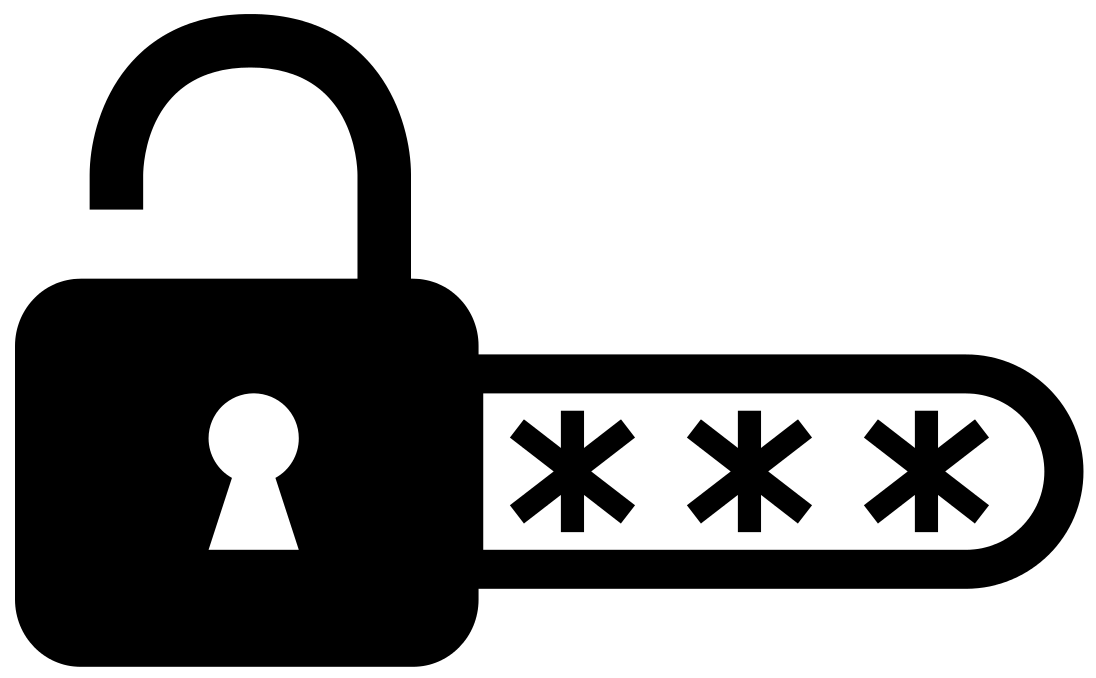
\includegraphics[width=0.2\textwidth]{password}};
                    \node[circle,draw,fill=gray,minimum width=4cm,anchor=215]
                    (have) at (0,1) {
                        
\includegraphics[height=0.2\textwidth]{phone}};
                    \node[circle,draw,fill=gray,minimum width=4cm,anchor=90]
                    (are) at (0,1) {
                        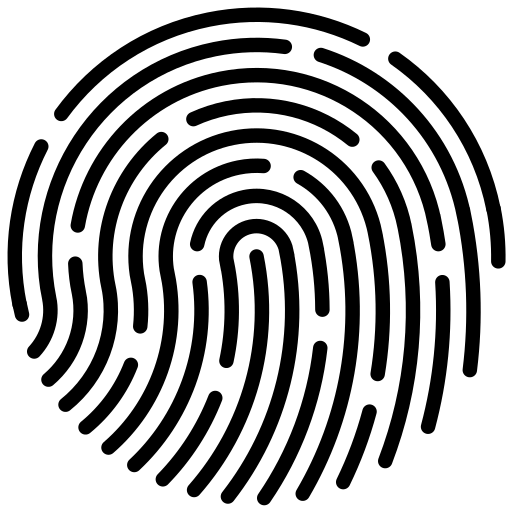
\includegraphics[height=0.2\textwidth]{touch-id}};
                \end{scope}
            \end{tikzpicture}
            \caption{Verschiedene Möglichkeiten für 2FA
                \endnote{\url{https://www.pngegg.com/en/png-eyxan}}
                \endnote{\url{https://images.vexels.com/media/users/3/157570/isolated/lists/4b39b362c76ea5a00de62f8ff839b5ed-einfaches-smartphone-symbol.png}}
                \endnote{\url{https://cdn4.iconfinder.com/data/icons/apple-touch-id/512/Touch_ID-512.png}}
            }
        \end{figure}
    \end{center}

    \note{
        \begin{itemize}
            \item Ungefähre Vorstellung, was alles 2FA ist, trotzdem kurze Definition\ldots
            \item Bei 2FA muss Nutzer 2 von 3 Faktoren vorzeigen, um sich zu authentifizieren
            \item Die Drei Faktoren sind
            \begin{itemize}
                \item etwas was man weiß \textrightarrow{} meistens ein Passwort
                \item etwas was man besitzt \textrightarrow{} zum Beispiel ein Handy oder ein zusätzliches Gerät
                \item etwas was man ist \textrightarrow{} also zum Beispiel Fingerabdruck oder Iris Scan
            \end{itemize}
            \item Kombination aus 2 würde man dann als 2FA bezeichnen
        \end{itemize}
    }
\end{frame}
